Il bottone "\textit{Pupil-Tracking}" (vedi figura \ref{fig:nerdmodelayout}) è abilitato solo qualora sia già in esecuzione l'analisi dell'immagine.

La funzionalità di "\textit{Pupil-Tracking}" acquisisce per ogni occhio rilevato dalla fase di analisi dell'immagine un occhio e su questa porzione di immagine avvia il rilevamento della pupilla.

Al termine del processamento della rete per il riconoscimento della pupilla (vedi \ref{sec:gazedetection}) i risultati vengono mostrati a video nelle stesse modalità di quelle descritte per "\textit{Eye-Tracking}".

Qui di seguito un test effettuato direttamente su Android Studio:

\begin{figure}[htbp]
    \centering
    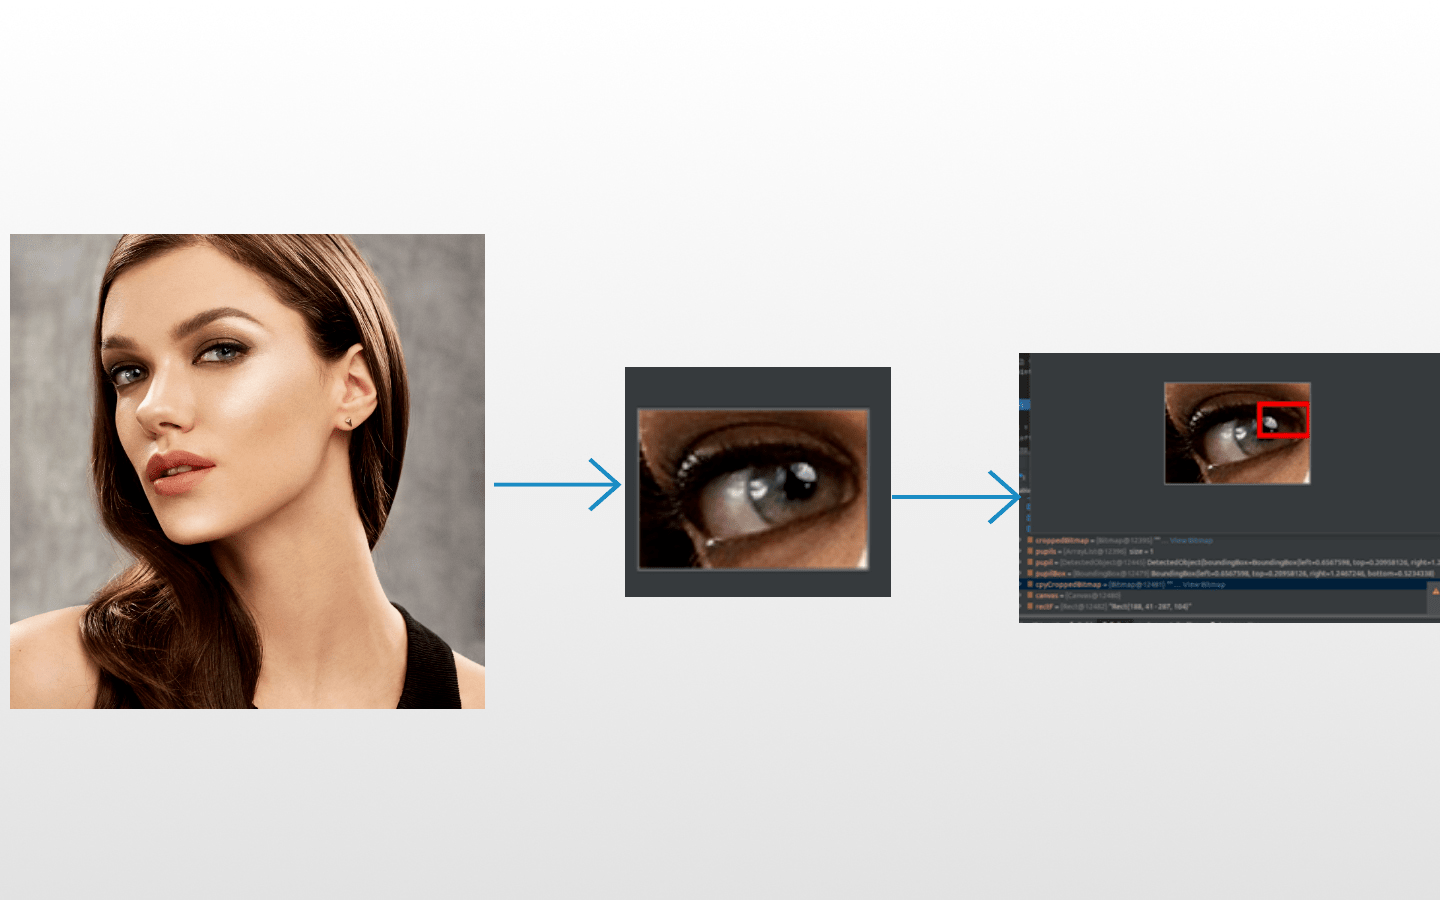
\includegraphics[scale=0.24]{ProgettoAndroid/NerdMode/RiconoscimentoPupilla/Images/gazeAndroid.png}
    \caption{Schermata Nerd mode con pupilla}
    \label{fig:nerdmodepupil}
\end{figure}